\section{Wstęp teoretyczny}
\subsection{Klasyfikacja}
\subsubsection{Klasyfikator kNN (k-najbliższych sąsiadów) \cite{wyklad}}
Klasyfikator kNN, ze względu na swoją intuicyjność, jest jednym z najpopularniejszych klasyfikatorów. Działa on zgodnie z regułą: obserwacja x zostaje sklasyfikowana do najliczniejszej klasy z pośród k obserwacji najbliższych punktowi x.\\

Szacowane prawdopodobieństwo przynależności obserwacji ${x}$ do danej klasy wśród ${x}$ najbliższych sąsiadów, zapisujemy jako:

\begin{equation}
    \hat{j}|\mathbf{x} = \frac{1}{k} \sum_{i=1}^{n} l\left( \rho(\mathbf{x}, \mathbf{x}_i) \leq \rho(\mathbf{x}, \mathbf{x}^{(k)}) \right) l(y_i = j), \quad j = 1, \ldots, g
\end{equation}

gdzie:\\
${x}^{(k)}$ - jest k-tym co do odległości ${x}$ punktem z próby uczącej\\
$\rho$ - jest pewną odległością, określaną jako miara niepodobieństwa.

\subsubsection{Naiwny Klasyfikator Bayesa \cite{wyklad}}
Jest klasyfikatorem probabilistycznym, który opiera się na użyciu twierdzenia.

\begin{equation}
P(C|F_1, \ldots, F_n)
\end{equation}

gdzie:\\
$C$ - oznacza zmienną zależną, będącą zbiorem etykiet klas\\
 $F_1, \ldots, F_n$ - cechami opisującymi zbiór przypadków.\\

 Korzystając z twierdzenia Bayesa, które mówi że dla dowolnej hipotezy $h \in \mathcal{H}$ oraz zbioru danych D zachodzi równość:

\begin{equation}
    P(h|D) = \frac{P(h) P(D|h)}{P(D)}
\end{equation}

oraz niezależności warunkowej cech $F_i$ oraz $F_j$ dla $i \neq j$ otrzymujemy:
\begin{equation}
    P(F_i|C, F_j) = P(F_i|C)
\end{equation}
Co ostatecznie daje:\\

\begin{equation}
    P(C|F_1, \ldots, F_n) = \frac{1}{Z} P(C) \prod_{i=1}^n P(F_i|C)
\end{equation}
przy czym $Z$ oznacza współczynnik skalujący, zależny od atrybutów $F_1, \ldots, F_n$ i ustalony w przypadku znanych wartości atrybutów cech.\\
    
Zatem wynik działania naiwnego klasyfikatora bayesowskiego można zapisać jako:
\begin{equation}
    \text{klasa}(f_1, \ldots, f_n) = \arg\max_c P(C = c) \prod_{i=1}^n P(F_i = f_i | C = c)
\end{equation}

\subsubsection{SVM - Maszyna Wektorów Nośnych \cite{svm_wiki} \cite{wyklad}}
Maszyna Wektorów Nośnych (Maszyna Wektorów Wspierających) jest to abstrakcyjny koncept maszyny, która działa jak klasyfikator, a której nauka ma na celu wyznaczenie hiperpłaszczyzny rozdzielającej z maksymalnym marginesem przykłady należące do dwóch klas.\\

Zadanie sprowadza się do znalezienia granicy decyzyjnej między klasami i związane jest z pojęciem separowalności liniowej, zgodnie z którym dwie klasy są liniowo separowalne, gdy istnieje hiperpłaszczyzna $H$ postaci $g(x)$ wyrażona równaniem:
\begin{equation}
    g(\mathbf{x}) = \mathbf{w}^T \mathbf{x} + b.
\end{equation}
    przyjmująca wartości:
\begin{equation}
    \begin{cases}
    g(\mathbf{x}_i) > 0 & \text{jeśli } \mathbf{x}_i \in 1, \\
    g(\mathbf{x}_i) < 0 & \text{jeśli } \mathbf{x}_i \in -1
    \end{cases}
\end{equation}
    gdzie: $\mathbf{x}$ - oznacza wektor danych, zaś $\mathbf{w}$ oraz $b$ są parametrami modelu.\\

W rezultacie można uzyskać zbiór wielu możliwych rozwiązań (czyli hiperpłaszczyzn), z których wybierane jest takie, które maksymalizuje margines klasyfikatora liniowego:\\
\begin{figure}[h]
    \centering
    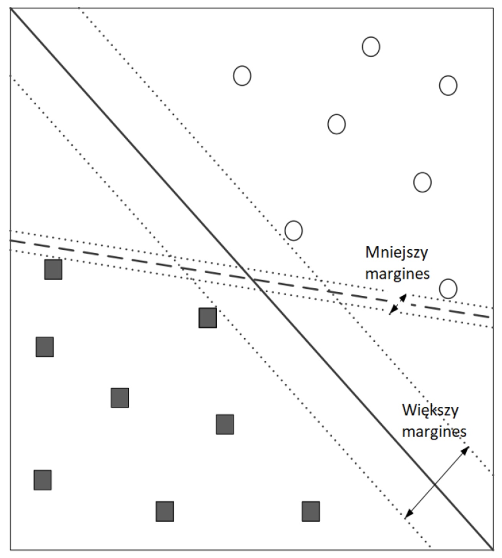
\includegraphics[scale=0.8]{svm}
    \caption{Schemat działania SVM}
    \label{fig:svm}
\end{figure}\\
Powyższy rysunek przedstawia uproszczony schemat działania SVM - źródło: materiały wykładowe.

\subsection{Ewaluacja modelu klasyfikacyjnego}
\subsubsection{Macierz pomyłek \cite{wyklad}}
Macierz pomyłek (błędów, ang. confusion matrix), inaczej określana mianem tablicy kontyngencji (ang. contingency table). prezentuje liczby przypadków należących do poszczególnych poprawnych klas decyzyjnych oraz tych, które są przewidywane.\\

W przypadku wielu etykiet macierz pomyłek jest macierzą kwadratowa m x m:\\


\begin{table}[h!]
    \centering
    \begin{tabular}{|c|c|c|c|c|}
    \hline
     & Class$_1$ & Class$_2$ & \ldots & Class$_m$ \\
    \hline
    Class$_1$ & $n_{11}$ & $n_{12}$ & \ldots & $n_{1m}$ \\
    \hline
    Class$_2$ & $n_{21}$ & $n_{22}$ & \ldots & $n_{2m}$ \\
    \hline
    \vdots & \vdots & \vdots & \vdots & \vdots \\
    \hline
    Class$_m$ & $n_{m1}$ & $n_{m2}$ & \ldots & $n_{mm}$ \\
    \hline
    \end{tabular}
    \end{table}
    
\noindent W klasyfikacji wieloklasowej oznaczamy często tylko jedną klasę jako pozytywną, a pozostałe łącznie definiujemy jako negatywne - sprowadzając problem do wielu klasyfikacji binarnych.

\subsubsection{Walidacja krzyżowa}
W związku z tym że wykorzystany wzór nie jest zbiorem zbyt licznym warto zastosować tzn. walidację krzyżową (inaczej kroswalidację, ang. \textit{cross-validation}).\\

\begin{enumerate}
    \item K-krotna walidacja krzyżowa polega na podzieleniu całego zbioru przypadków na k
rozłącznych i równolicznych części
    \item Kolejno każda z tych części stanowi wydzielony zbiór testowy, a pozostałe k-1 - zbiór uczący.
    \item Walidację przeprowadza się na każdej z k części zbioru, zaś wynik końcowy jest średnią z poszczególnych wyników częściowych.
\end{enumerate}

\subsubsection{Pozostałe podstawowe metryki}
W pracy wykorzystano również: dokładność (\textit{Accuracy}), precyzja (\textit{Precision}), czułość (\textit{Sensitivity}), specyficzność (\textit{Specificity}) oraz predykcję klasy negatywnej (\textit{Negative Predictive Value}). 

\subsection{Sztuczne sieci neuronowe}
\subsubsection{Perceptron wielowarstwowy}
Perceptron wielowarstwowy (MLP, ang. \textit{Multi-Layer Perceptron}) jest podstawowym typem sztucznej sieci neuronowej, który składa się z co najmniej trzech warstw: warstwy wejściowej, jednej lub więcej warstw ukrytych oraz warstwy wyjściowej. Każdy neuron w jednej warstwie jest połączony z każdym neuronem w warstwie następnej, co umożliwia przetwarzanie skomplikowanych wzorców i zależności. W przeciwieństwie do prostego perceptronu jednopoziomowego, MLP jest zdolny do rozwiązywania problemów, które nie są liniowo separowalne. Proces uczenia w MLP opiera się na algorytmie wstecznej propagacji błędów, który minimalizuje błąd sieci poprzez dostosowanie wag połączeń między neuronami. Perceptrony wielowarstwowe są powszechnie stosowane w zadaniach takich jak klasyfikacja, regresja oraz rozpoznawanie wzorców. Ze względu na swoją elastyczność i moc obliczeniową, MLP stanowi fundament dla bardziej zaawansowanych struktur sieci neuronowych, takich jak sieci konwolucyjne i rekurencyjne. Jego zdolność do uczenia się nieliniowych relacji sprawia, że jest to narzędzie niezwykle użyteczne w szerokim zakresie zastosowań, od rozpoznawania obrazów po przetwarzanie języka naturalnego.

\subsubsection{Sieci głębokie}
Sieci głębokie (ang. Deep Neural Networks, DNN) to zaawansowane struktury sztucznych sieci neuronowych, które charakteryzują się dużą liczbą warstw ukrytych pomiędzy warstwą wejściową a wyjściową. Dzięki wielowarstwowej architekturze, sieci głębokie mogą modelować bardzo złożone i nieliniowe relacje w danych. Proces uczenia tych sieci wykorzystuje zaawansowane techniki, takie jak wsteczna propagacja błędów oraz optymalizatory gradientowe, które umożliwiają skuteczne dostosowanie wag neuronów. Sieci głębokie są niezwykle efektywne w zadaniach związanych z przetwarzaniem dużych ilości danych, takich jak rozpoznawanie obrazów, analiza dźwięku czy przetwarzanie języka naturalnego. Wprowadzenie warstw konwolucyjnych i rekurencyjnych w ramach sieci głębokich dodatkowo rozszerza ich możliwości, umożliwiając analizę sekwencji i wykrywanie istotnych wzorców w danych przestrzennych. Rozwój technologii sprzętowych, takich jak GPU, oraz technik takich jak dropout, znacząco przyczynił się do sukcesu i szerokiego zastosowania sieci głębokich. Dzięki swojej zdolności do automatycznego ekstraktowania cech i wysokiej dokładności predykcji, sieci głębokie stanowią fundament współczesnej sztucznej inteligencji i uczenia maszynowego.

\subsubsection{Funkcja aktywacji softmax}
Funkcja aktywacji softmax jest powszechnie stosowana w sieciach neuronowych, szczególnie w warstwach wyjściowych modeli klasyfikacyjnych, aby przekształcić surowe wartości wyjściowe neuronów w prawdopodobieństwa. Softmax przekształca wektor wartości rzeczywistych w wektor wartości, które sumują się do 1, co umożliwia interpretację wyniku jako rozkład prawdopodobieństwa między różnymi klasami. Wartości wyjściowe są eksponowane i następnie normalizowane, co podkreśla różnice między nimi i pomaga w dokładniejszej klasyfikacji. Dzięki swoim właściwościom, funkcja softmax jest idealna do zadań wieloklasowej klasyfikacji, gdzie model musi przypisać jedno z wielu możliwych oznaczeń do danego wejścia.